%%%%%%%%%%%%%%%%%%%%%%%%%%%%%%%%%%%%%%%%%
% Programming/Coding Assignment
% LaTeX Template
%
% This template has been downloaded from:
% http://www.latextemplates.com
%
% Original author:
% Ted Pavlic (http://www.tedpavlic.com)
%
% Note:
% The \lipsum[#] commands throughout this template generate dummy text
% to fill the template out. These commands should all be removed when 
% writing assignment content.
%
% This template uses a Perl script as an example snippet of code, most other
% languages are also usable. Configure them in the "CODE INCLUSION 
% CONFIGURATION" section.
%
%%%%%%%%%%%%%%%%%%%%%%%%%%%%%%%%%%%%%%%%%

%----------------------------------------------------------------------------------------
%	PACKAGES AND OTHER DOCUMENT CONFIGURATIONS
%----------------------------------------------------------------------------------------
\documentclass{article}

\usepackage{fancyhdr} % Required for custom headers
\usepackage{lastpage} % Required to determine the last page for the footer
\usepackage{extramarks} % Required for headers and footers
\usepackage[usenames,dvipsnames]{color} % Required for custom colors
\usepackage{graphicx} % Required to insert images
\usepackage{listings} % Required for insertion of code
\usepackage{courier} % Required for the courier font
\usepackage{pgfgantt}
\usepackage{amsmath}
\usepackage{mathabx}
\usepackage{mathtools}
\usepackage{qtree}
\usepackage{multicol}



% Margins
\topmargin=-0.45in
\evensidemargin=0in
\oddsidemargin=0in
\textwidth=6.5in
\textheight=9.0in
\headsep=0.3in

\linespread{1.1} % Line spacing

% Set up the header and footer
\pagestyle{fancy}
\lhead{\homeworkProblemName} % Top left header
\chead{} % Top center head
\rhead{\hmwkClass} % Top right header
\lfoot{\textit{\homeworkSectionName}} % Bottom left footer
\cfoot{} % Bottom center footer
\rfoot{Page\ \thepage\ of\ \protect\pageref{LastPage}} % Bottom right footer
\renewcommand\headrulewidth{0.4pt} % Size of the header rule
\renewcommand\footrulewidth{0.4pt} % Size of the footer rule

\setlength\parindent{0pt} % Removes all indentation from paragraphs

%----------------------------------------------------------------------------------------
%	CODE INCLUSION CONFIGURATION
%----------------------------------------------------------------------------------------

\definecolor{MyDarkGreen}{rgb}{0.0,0.4,0.0} % This is the color used for comments
\lstloadlanguages{Java} % Load Java syntax for listings, for a list of other languages supported see: ftp://ftp.tex.ac.uk/tex-archive/macros/latex/contrib/listings/listings.pdf
\lstset{language=Java, % Use Java in this example
        frame=none, % Single frame around code
        basicstyle=\small\ttfamily, % Use small true type font
        keywordstyle=[1]\color{Blue}\bf, % Perl functions bold and blue
        keywordstyle=[2]\color{Purple}, % Perl function arguments purple
        keywordstyle=[3]\color{Blue}\underbar, % Custom functions underlined and blue
        identifierstyle=, % Nothing special about identifiers                                         
        commentstyle=\usefont{T1}{pcr}{m}{sl}\color{MyDarkGreen}\small, % Comments small dark green courier font
        stringstyle=\color{Purple}, % Strings are purple
        showstringspaces=false, % Don't put marks in string spaces
        tabsize=8, % 5 spaces per tab
        %
        % Put standard Perl functions not included in the default language here
        morekeywords={rand},
        %
        % Put Perl function parameters here
        morekeywords=[2]{on, off, interp},
        %
        % Put user defined functions here
        morekeywords=[3]{test},
       	%
        morecomment=[l][\color{Blue}]{...}, % Line continuation (...) like blue comment
        numbers=left, % Line numbers on left
        firstnumber=1, % Line numbers start with line 1
        numberstyle=\tiny\color{Blue}, % Line numbers are blue and small
        stepnumber=100 % Line numbers go in steps of 5
}


%----------------------------------------------------------------------------------------
%	DOCUMENT STRUCTURE COMMANDS
%	Skip this unless you know what you're doing
%----------------------------------------------------------------------------------------

% Header and footer for when a page split occurs within a problem environment
\newcommand{\enterProblemHeader}[1]{
\nobreak\extramarks{#1}{#1}\nobreak
\nobreak\extramarks{#1}{#1}\nobreak
}

% Header and footer for when a page split occurs between problem environments
\newcommand{\exitProblemHeader}[1]{
\nobreak\extramarks{#1}{#1 continued on next page\ldots}\nobreak
\nobreak\extramarks{#1}{}\nobreak
}

\setcounter{secnumdepth}{0} % Removes default section numbers
\newcounter{homeworkProblemCounter} % Creates a counter to keep track of the number of problems

\newcommand{\homeworkProblemName}{}
\newenvironment{homeworkProblem}[1][
 \arabic{homeworkProblemCounter}]{ % Makes a new environment called homeworkProblem which takes 1 argument (custom name) but the default is "Problem #"
\stepcounter{homeworkProblemCounter} % Increase counter for number of problems
\renewcommand{\homeworkProblemName}{#1} % Assign \homeworkProblemName the name of the problem
\section{\homeworkProblemName} % Make a section in the document with the custom problem count
\enterProblemHeader{} % Header and footer within the environment
}{
\exitProblemHeader{} % Header and footer after the environment
}

\newcommand{\problemAnswer}[1]{ % Defines the problem answer command with the content as the only argument
\noindent\framebox[\columnwidth][c]{\begin{minipage}{0.98\columnwidth}#1\end{minipage}} % Makes the box around the problem answer and puts the content inside
}

\newcommand{\homeworkSectionName}{}
\newenvironment{homeworkSection}[1]{ % New environment for sections within homework problems, takes 1 argument - the name of the section
\renewcommand{\homeworkSectionName}{#1} % Assign \homeworkSectionName to the name of the section from the environment argument
\subsection{\homeworkSectionName} % Make a subsection with the custom name of the subsection
\enterProblemHeader{\homeworkProblemName\ [\homeworkSectionName]} % Header and footer within the environment
}{
\enterProblemHeader{\homeworkProblemName} % Header and footer after the environment
}

%my commands
\newcommand{\dent}{\qquad\qquad}


%----------------------------------------------------------------------------------------
%	NAME AND CLASS SECTION
%----------------------------------------------------------------------------------------

\newcommand{\hmwkTitle}{Final Year Project Report} % Assignment title
\newcommand{\hmwkDesc}{A thesis submitted in part fulfilment of the degree of\\
\textbf{BSc. (Hons.) in Computer Science}} % Due date
\newcommand{\hmwkClass}{A Theorem Proving Assistant} % Course/class
\newcommand{\hmwkClassTime}{} % Class/lecture time
\newcommand{\hmwkClassInstructor}{Interim Report} % Teacher/lecturer
\newcommand{\hmwkAuthorName}{Joe Duffin} % Your name

%----------------------------------------------------------------------------------------
%	TITLE PAGE
%----------------------------------------------------------------------------------------

\title{
\vspace{0.3in}
\textbf{\hmwkTitle}
\vspace{1in}\\
\textmd{\textbf{\hmwkClass}}\\\ \\
\normalsize\
\vspace{0.4in}
\textmd{\textbf{\hmwkAuthorName}}\\
\vspace{0.1in}
\small{\hmwkDesc}\\
\vspace{0.05in}
\small{\textbf{Supervisor}: Henry Mcloughlin}
\vspace{.5in}
\begin{center}

\includegraphics[width=0.3\columnwidth]{UCD_Logo} % Example image
\end{center}
}


\author{School of Computer Science\\University College Dublin}


\date{\small{November 5, 2016}} % Insert date here if you want it to appear below your name

%use dash as list marker
\def\labelitemi{--}
%----------------------------------------------------------------------------------------

\begin{document}
\begin{titlepage}
\maketitle
\thispagestyle{empty}
\end{titlepage}

\newpage
%----------------------------------------------------------------------------------------
%	TABLE OF CONTENTS
%----------------------------------------------------------------------------------------

%\setcounter{tocdepth}{1} % Uncomment this line if you don't want subsections listed in the ToC

\newpage
\tableofcontents

\newpage

%----------------------------------------------------------------------------------------
\begin{homeworkProblem}[Project Specification]
\begin{description}

\item \textbf{General Information}\\
Calculational Theorem Proving is the name given to a particular style of mathematical proof which
was developed during the 1980s by Feijen and Dijkstra. It emphasises the syntactic manipulation
of expressions rather than manipulation based on an interpretation of the expression. In doing so it tries to let the notation do the work.\\

In order to do so the choice of notation and they layout of the proofs are important.\\

This style of proof has been taught in a number of our undergraduate modules over the last 10
years and is probably quite familiar to all of our undergraduates. An example proof would have
been included here but the special symbols for the boolean operators were not available.\\

The aim of this project is to develop a tool which will assist the person proving the theorem
by performing basic housekeeping tasks. So for example, the user should be able to select a
sub-expression, select an appropriate rule to transform it, and have the system carry out the
transformation and record the appropriate hint to show which rule was used and what the variable bindings were. It is important to mention that we are not interested in automatic theorem proving, the user will still be required to drive the proof but the system will perform the matching and applying of the rules.\\

It should be possible to store and retrieve partial or complete proofs. It should be possible to undo a series of steps and select different rules to apply. Once a theorem is proved it should be possible to add it to the rule base so it can be used in future proofs.

\item \textbf{Mandatory Requirements}\\
$\circ$ The design of algorithms to a selected sub-expression with a subexpression of a rule.\\
$\circ$ The design of an interface to allow users to select subexpressions and rules to apply.\\
$\circ$ The design of appropriate algorithms to allow partial and complete proofs to be stored and retrieved.\\
$\circ$ The design of appropriate algorithms to allow the user to undo steps in a proof.\\
$\circ$ The implementation of the above functionality.

\item \textbf{Discretionary Requirements}\\
$\circ$ Incorporating quantified expressions and their manipulation rules in the system.

\item \textbf{Exceptional Requirements}\\
$\circ$ Incorporating additional small calculii such as Max/Min, Floor/Ceiling and GCD/LCM into the system.

\item \textbf{Suggested Reading}\\
$\circ$ http://www.cs.utexas.edu/~EWD/\\
$\circ$ http://www.mathmeth.com/\\
$\circ$ Program Construction by Roland Backhouse\\
$\circ$ A logical approach to discrete maths by David Gries
\end{description}

\newpage
\end{homeworkProblem}
%----------------------------------------------------------------------------------------

\begin{homeworkProblem}[Abstract]

\begin{description}
\item \textbf{Context}\\
This report introduces the reader to predicate calculus and theorem proving in the style used by Dijkstra. It highlights the features of it that lend themselves to a computer application. Proving boolean theorems is a pattern matching excersise without need for interpretation of the expression at each stage of the proof. This report explores issues and solutions for building software package which facilitates theorem proving in a clear and easy manor.

\item \textbf{Methodology}\\
An exploratory approach was taken to not only resolving the major issues but finding them aswell. There is no road map to follow so a lot of time and resources were put into paths that led nowhere. In order to carry out this project I have had to define algorithms which are relied upon throughout, some of which have proven to be flawed and others invaluable. I shall discuss these. 

\item \textbf{Findings}\\
At this stage of the project I believe that the major fundamental building blocks are in place. I have defined ways of representing expressions and carrying out steps of a proof. Simple pattern matching and replacement excersises can be conducted programatically. The algorithms used will be discussed indepth.\end{description}

\newpage
\end{homeworkProblem}

%----------------------------------------------------------------------------------------

\begin{homeworkProblem}[Acknowledgments]
Thank you kindly
\newpage
\end{homeworkProblem}

%----------------------------------------------------------------------------------------
\begin{homeworkProblem}[Introduction to Predicate Calculus]
Predicate calculus works like this: given a set of axioms and theorems (rules) one can calculate, or derive, further theorems. Relying on those derived previously a full calculus can be evolved. This process relies heavily on pattern matching and this notion is vitaly important. With each step of a proof a hint is given which tells the reader which rule was used and what assignment was made to each variable in that rule. Dijykstra states that the notation used is vitally important for a clear and easy to read proof \cite{DIJKSTRA:1990}.\\
\begin{homeworkSection}{Prelimniaries}
Before giving an example proof we must set some conventions for notation and give information about operators. 
\begin{itemize}
\item Upper case letters such as $X$,$Y$ and $Z$ will be used as boolean identifiers.
\item For this report I am only going to introduce 3 operators:
\begin{description}
\item \textbf{Conjunction }(boolean and): $\wedge$ 
\item \textbf{Disjunction }(boolean or): $\vee$ 
\item \textbf{Equivalence }(boolean equals): $\equiv$
\end{description}
\item Equivalence holds the lowest precedence of the three operators and conjunction and disjunction share equal precedence meaning explicit bracketing must sometimes be used.
\item Brackets can be introduced as long as precedence and operators operands are respected.
\item Brackets can be removed from unary expressions.
\item Rules will be numbered and named and be referenced to by their number or name.
\item Each new line of a proof will be preceeded by an assignment and the corresponding rule. We call this "the hint".\\
eg. $\{(X,Y\coloneqq Z,Y).(5)\}$ reads as $X$ and $Y$ are assigned the values $Z$ and $Y$ respectively in rule 5.
\item Axioms will be denoted with a $*$ to the left of it's number and theorems with a $\cdot$.
\end{itemize}
\vspace{0.5cm}
In order to give a sample proof I provide the following set of axioms and theorems.
\begin{align*}
&*\ (0)\ [(X\equiv (Y\equiv Z))\equiv ((X\equiv Y)\equiv Z)]&\equiv \text{ associative}\\
&*\ (1)\ [X\equiv Y\equiv Y \equiv X]&\equiv \text{ symmeetric}\\
&*\ (2)\ [X \equiv true \equiv X ]&\equiv \text{ identity}\\
&\cdot\ (3)\ [X \equiv X]&\equiv \text{ reflexive}\\
&\cdot\ (4)\ [true]&\text{true}\\
&*\ (5)\ [X \vee Y \equiv Y \vee X]&\vee \text{ symmetric}\\
&*\ (6)\ [X \vee (Y\vee Z) \equiv (X\vee Y) \vee Z]&\vee \text{ associative}\\
&*\ (7)\ [X \vee X \equiv X]&\vee \text{ idempotent}\\
&*\ (8)\ [X \vee (Y \equiv Z) \equiv X \vee Y \equiv X \vee Z]&\vee /\equiv 
\end{align*}
\newpage
\end{homeworkSection}

\begin{homeworkSection}{A Sample Proof}
We will now attempt to prove that disjuntion distributes over its self.
\begin{align*}
&(X\vee Y) \vee (X \vee Z) \\
=&\dent \{(X,Y,Z\coloneqq (X\vee Y),X,Z).(6)\}\\
&((X\vee Y) \vee X) \vee Z \\
=&\dent \{(X,Y\coloneqq (X\vee Y),X)).(5)\}\\
&(X \vee (X\vee Y)) \vee Z \\
=&\dent \{(X,Y,Z\coloneqq (X,X,Y).(6)\}\\
&((X \vee X)\vee Y) \vee Z \\
=&\dent \{(X\coloneqq X).(7)\}\\
&((X)\vee Y) \vee Z \\
=&\dent \{remove\ brackets\}\\
&(X\vee Y) \vee Z \\
=&\dent \{(X,Y,Z\coloneqq (X,Y,Z).(6)\}\\
&X\vee (Y \vee Z)\\
\end{align*}
This  has yielded a new theorem so we shall record it so it is available for use in future proofs.
\begin{align*}
&\cdot\ (9)\ [(X \vee Y) \vee (X \vee Z) \equiv X\vee (Y \vee Z)]&\vee/\vee
\end{align*}
Note that in the above proof no interpretation of any of the boolean expressions was done. It is purely a pattern matching exercise. At each step of the proof we used a single theorem to replace a section of an expression with an equivalent section. I plan to build a theorem proving assistant by exploiting this feature of the proof style.\\
\newpage
\end{homeworkSection}

\end{homeworkProblem}
%----------------------------------------------------------------------------------------
\begin{homeworkProblem}[Introduction to This Report]

\begin{homeworkSection}{What I intend to build}
The theorem proving assistant will provide a user friendly software environment for assisting in proving predicate calculus theorems. It will not be an automated tool, but one which provides the user with a comprehensive and robust environment in which theorems can be proved. The software will take care of the "housework", such as automating the generation of the hint between each step.\\

The user will be presented with an environment in which they prove theorems. In order to permute an expression the following steps will be carried out by the user:
\begin{enumerate}
\item Select a theorem (or sub-expression of a theorem) to use as the current expression.
\item Select a sub-expression in the current expression (the software will ensure that only a valid subexpression can be chosen).
\item Choose a theorem to apply.
\item Make a selection of which replacement/assigment to use from that theorem.
\item View the new expression generated with a hint step describing which theorem and what assigment was used.
\item Continue to permute the new expression as the current expression until a conclusion has been drawn.
\item Save the proven theorem as a new theorem for future use.
\end{enumerate}
Further functionality will also provide the user with the ability to define their own workspaces where a parser will be used to transalate a psuedo language into a set boolean expressions to be used as theorems. This parser will translate input such as "X and Y" into the expression "$X \wedge Y$" in a format that the software can use.
\newpage
\end{homeworkSection}

\begin{homeworkSection}{What I hope it will look like}
The interface will consist of two distinct areas. The left hand side is where the current expression and all steps taken to derive it will be displayed. It is here that a user will select a sub-expression of the current expression as described in step 2 above.\\

The righthand side of the interface will contain a list of numbered theorems. This list will be made up of loaded axioms as well as theorems that have been previously derived and saved by the user. It is here that a theorem will be chosen as described in step 3 above. The user will also have the ability to explore a theorem. This "exploration" will demonstrate from which theorem it was derived and which steps were taken in its derviation.\\

A button exists to move a theorem from the right hand side to the left hand side to start work and also a button to save the current expression as a theorem on the right hand side.
The entire workspace state will be able to be saved at any moment and returned to for further work.\\

\begin{center}
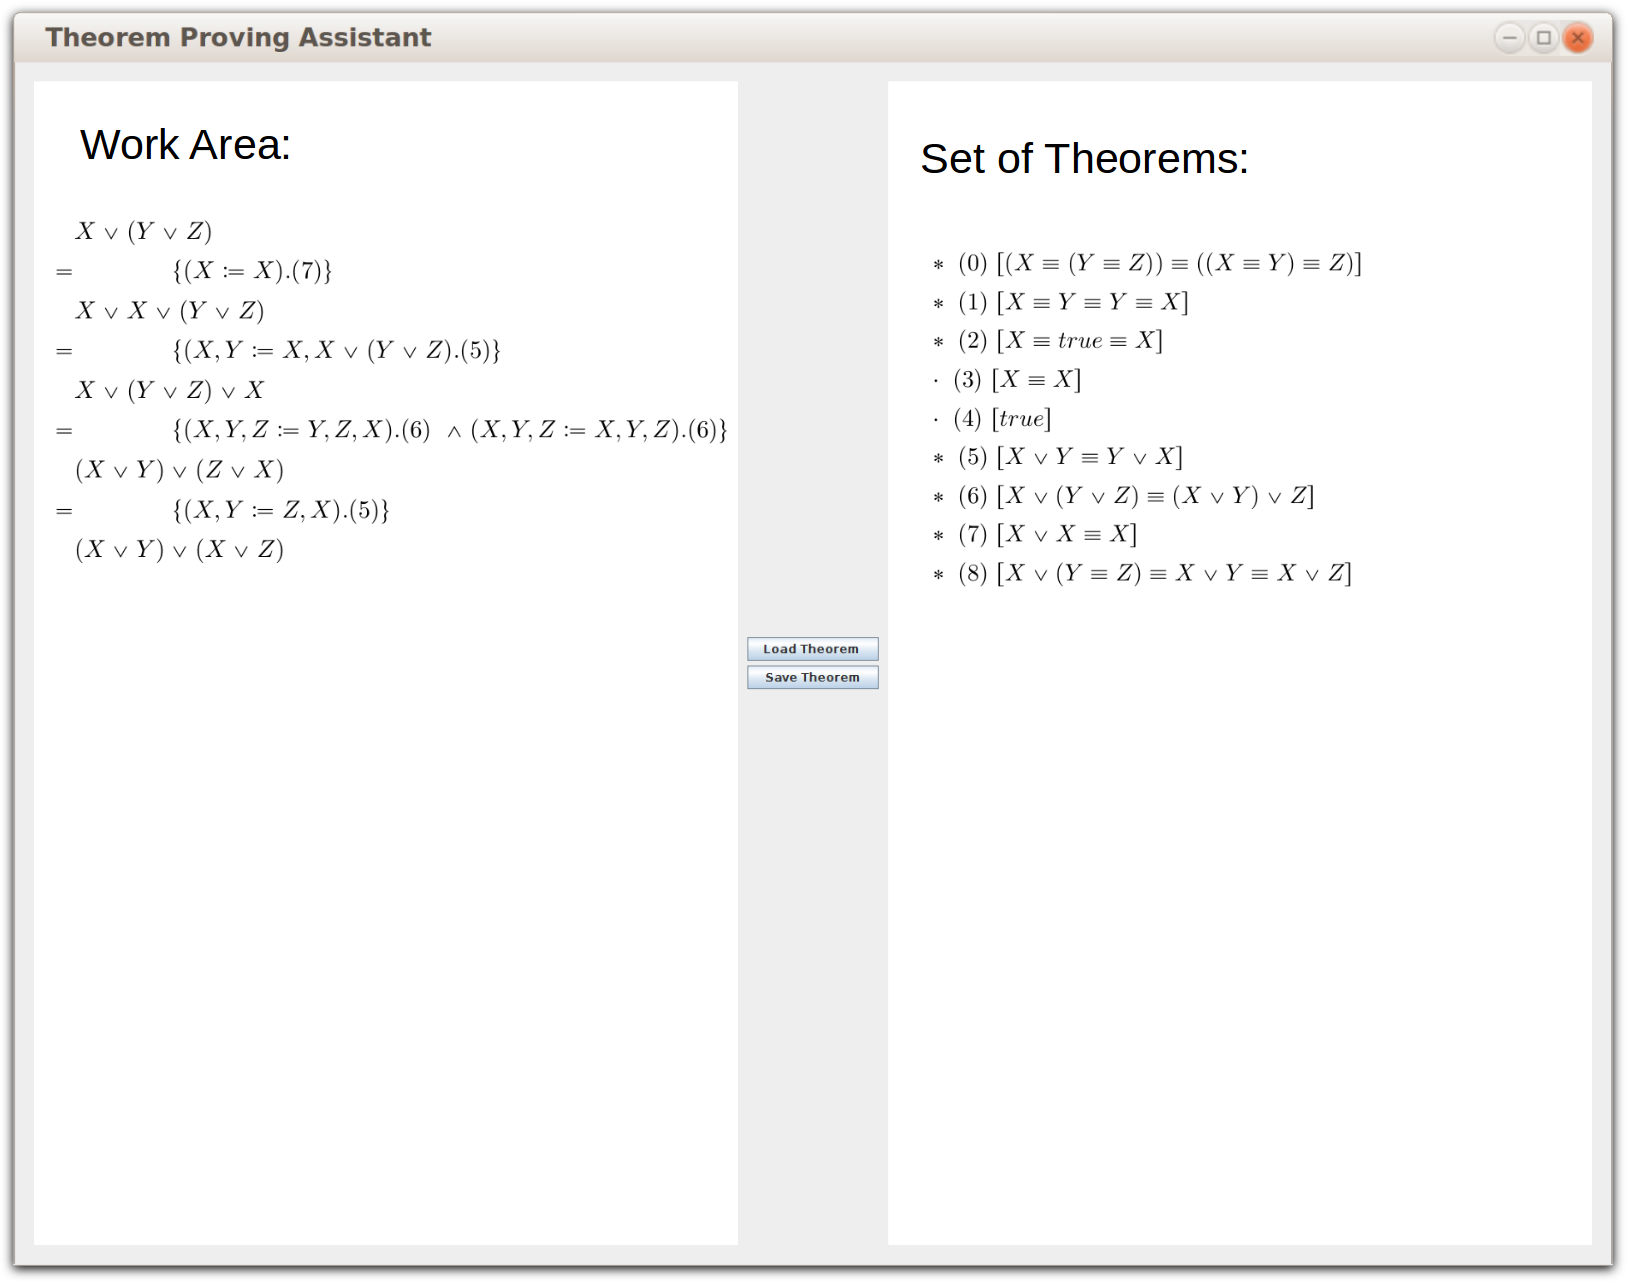
\includegraphics[width=1\columnwidth]{swag} % Example image
\end{center}
\newpage
\end{homeworkSection}



\end{homeworkProblem}


%----------------------------------------------------------------------------------------
\begin{homeworkProblem}[Functionality Overview]

yada 

\begin{homeworkSection}{User Experiance}
great
\newpage
\end{homeworkSection}

\begin{homeworkSection}{A highlevel of what actually happens}
whoosh
\newpage

\end{homeworkSection}
\end{homeworkProblem}

%----------------------------------------------------------------------------------------

\begin{homeworkProblem}[Backend Algorithms]


Here I present work completed so far.

\begin{homeworkSection}{Expression Representation}

When starting this project the only fact that was clear was the need to not represent expressions as strings. Immidiate issues associated with a string based solution are the lack of sense of precededence, the lack of pivots to easily commute around and no easy way to identify the begining and end of bracketed sections. \\

Syntax trees are a commonly used solution \cite{ULLMAN:1986}. Leaves would be identifiers and nodes operators. Below I demonstrate an example with a simple boolean expression: $X\wedge Y \equiv Z$.\\

\Tree [.$\equiv$  [ X Y !{\qbalance} ].$\wedge$ Z ]\\

In order to yield the boolean expression from the tree we need only to perform an in-order travesal, printing the leaf or node's identifier or operator as we visit them. As a human we can read the expression from the tree by reading the identifiers and operators from left to right.\\

Depth is used to indicate precedence. One can see how precedence is maintained as the conjunction operator is at a deeper level than the equivalence. The two operators are commutative and swapping the left and right children of either node will yield an equivalent (in terms of ultimate value) tree. \\

Bracketing sections proved to be more of an issue. Below I demonstrate several options that were considerd with the boolean expresion $(X \wedge Y) \vee Z$. \\

\Tree [.$\vee$ [  [ ( ].X [ ) ].Y  !{\qbalance} ].$\wedge$ Z ]
\Tree [.$\vee$ [ (X Y) !{\qbalance} ].$\wedge$ Z ]
\Tree [.$\vee$ [ [ X Y !{\qbalance} ].$\wedge$ ].$()$ Z ]\\

The decision as to which option to use was made for me when I turned my attention the defining a valid substring.
\newpage
\end{homeworkSection}

\begin{homeworkSection}{A Valid Sub-expression}
A valid sub-expression is a fundamental part of the project. It is what a user will first select in order to carry out a replacement. For a sub-expression to be valid when selecting it we must respect precedence, bracketing and the number of operands associated with an operator. These requirements indicate that maybe a formal grammar will need to be defined but up until a parser is needed I wish to avoid this. I fear that having a grammar at this stage will steer me towards string based solutions. Initially I would like to stick to purely tree based solutions due to the issues associated with string manipulation.\\ 

To demonstrate valid and invalid sub-expressions of $X \wedge Y \equiv Z$ I present the table below. 

\begin{center}
\begin{tabular}{|c|c|}
\hline
Valid & Invalid \\
\hline
$X \wedge Y $ & $Y \equiv Z$\\
$X $ & $\wedge Y$\\
$Z $ & $ \equiv Z $\\

\hline
\end{tabular}
\end{center}


Validating the selection of a sub-expression has to be a simple task. After drawing some syntax trees it became clear that any node's subtree is a valid sub-expression. For this reason the right most bracket option was chosen. Any node of that tree can be selected and its subtree is a valid sub-expression. We list the valid sub-exressions of $(X \wedge Y) \vee Z$ beside the tree and the corrolation becomes clear.

\begin{multicols}{2}


\Tree [.$\vee$ [ [ X Y !{\qbalance} ].$\wedge$ ].$()$ Z ]\\
\begin{tabular}{|c|}
\hline
$(X \wedge Y) \vee Z$\\
\hline
$(X \wedge Y) \vee Z$\\
$(X \wedge Y)$\\
$X \wedge Y$\\
$X$\\
$Y$\\
$Z$\\
\hline
\end{tabular}

\end{multicols}




Initially this simple approach of using a node's subtree to define a sub-expression appeared comprehensive but when I went to extract all valid sub-expressions of an expression with associative operators I realised this was not possible. We use the expression $X \wedge Y \wedge Z$ to demonstrate this. Consider the following tree representation and list of valid sub-expressions as defined above.

\begin{multicols}{2}

\Tree [.$\wedge$ [ X Y !{\qbalance} ].$\wedge$ Z ]\\
\begin{tabular}{|c|}
\hline
$X \wedge Y \wedge Z$\\
\hline
$X \wedge Y \wedge Z$\\
$X \wedge Y$\\
$X$\\
$Y$\\
$Z$\\
\hline
\end{tabular}

\end{multicols}

$Y \wedge Z$ is a valid sub-expression of $X \wedge Y \wedge Z$ but is not attainable from the above tree in its current state. We need to permute the syntax tree to "re-shuffle" it so $Y \wedge Z$ can exist as a subtree while still maintaining the value of the boolean expression. 

\newpage
\end{homeworkSection}
\begin{homeworkSection}{Permutations of a Syntax Tree}

In order to achieve this re-shuffling of a tree we need to rely on a tree rotation algorithm called zigging \cite{GOODRICH:2010}. Performing the zig operation on the deeper conjunction node will rotate the tree clockwise, causing the node to be the new root. $X$ will be the left child of the new root with the previous root as its right child. The old roots right child, $Z$, persists, and the temporarily orphaned $Y$ becomes $Z$s sibling. The following two trees present two permutations of a tree for $X\wedge Y\wedge Z$ attainable by zigging the left or right child of the root.

\Tree [.$\wedge$ [ X Y !{\qbalance} ].$\wedge$ Z ] 
\Tree [.$\wedge$  X [ Y Z !{\qbalance} ].$\wedge$ ]\\

Now by unioning the the set of sub-expressions yielded from the two trees we have a complete set. This simple approach however does not scale. An algorithm combining commuting nodes, zigging nodes and zigging nodes from a depth of two is needed in order yield all valid sub-expressions of any tree. It is at this point that I must introduce the caveat that commutitivity is taken for granted. The algorithm will not only yield all sub-expressions permissisable by the associtivity of the operators, but also those permissable by the commutativity of the operators. Expressions such as $X \wedge Y$ and $ Y \wedge X$ will be considered equivalent.\\

Consider the following series of tree representations of $X \wedge Y \wedge Z \wedge W \wedge Q$ and one can see how the whole tree is being "dragged" through the root node by performing the zig operation on the roots left child.

\Tree [ .$\wedge$ [ [ [ X Y !{\qbalance} ].$\wedge$  Z ].$\wedge$ W  ].$\wedge$ Q ] 
\Tree [ .$\wedge$ [ [ X Y !{\qbalance} ].$\wedge$ Z ].$\wedge$ [ W Q !{\qbalance} ].$\wedge$ ]\ \ \ \ 
\Tree [ .$\wedge$  [ X Y !{\qbalance} ].$\wedge$ [ Z [ W Q !{\qbalance} ].$\wedge$ ].$\wedge$ ] 
\Tree [ .$\wedge$ X [ Y [ Z [ W Q ].$\wedge$ ].$\wedge$ ].$\wedge$ ]\\

After each zig if we either do or do not commute the roots children and continue until no new trees are generated we will create every possible permutation. When the alorithm stops we have will yielded all $5!$ equivalent tree permutations. The following tree is one of them which will be produced at some point during permuting algorithm (I am not going to list all $5!$ of them!).

\Tree [ .$\wedge$ [ Y W !{\qbalance} ].$\wedge$ [ [ X Z !{\qbalance} ].$\wedge$ Q ].$\wedge$ ]\\

Recursively calling the described permute algorithm on the children of the root of each permutation will ultimately yield all valid sub-expressions. When attempting to identify valid sub-expressions of an expression all permutations of that expressions's tree must exist simulatiously; all possible tree arrangments for a given expression must be considered when validating or refuting an operation on an expression.


\newpage
\end{homeworkSection}
\begin{homeworkSection}{Matching, Mapping and Replacing}

At this point I introduce a new theorem but no longer in terms of X and Y but P and Q.
\begin{align*}
&\cdot\ \ [P \wedge ( P \vee Q ) \equiv P]& absorbtion0
\end{align*}
We consider a state half way through a proof where the user's current expression is $X \wedge (X \vee Y ) \equiv X \wedge Y$ and wishes to use absorbtion0 to replace the entire left hand side of the expression with X. The action is documented below with the notation we defined.
\begin{align*}
&X \wedge (X \vee Y ) \equiv X \wedge Y  \\
=&\dent \{(P,Q\coloneqq X,Y).(absorbtion0)\}\\
&X \equiv X \wedge Y
\end{align*}

As humans we can easily map P to X and Q to Y and do the replacement as it is in our nature to look for patterns and repetition. To design alorithms for a computer to do this is an complex task. To further complicate the matter we change the the boolean identifier Y on the left hand side of the expression to a boolean expression consisting of several operands. We redine the current expression and application of absorbtion0 as follows.
\begin{align*}
&X \wedge (X \vee (Z \wedge W) ) \equiv X \wedge Y  \\
=&\dent \{(P,Q\coloneqq X,(Z \wedge W)).(absorbtion0)\}\\
&X \equiv X \wedge Y
\end{align*}

In looking to match the users selection ($X \wedge (X \vee (Z \wedge W) )$) with a sub-expression of absorbtion0 we must compare it to every valid sub-expression of absorbtion0. Not only that, but we must handle the fact that the boolean identifiers in the rule and current expression are completely different. We start by drawing a tree representation of the current expression with the current expression highlighted and the rule, absorbtion0. Note that I have convieniently chosen to draw the correct permutation the rule. A software program will have to itterate through all permutations in attempts to find matches. \\

Current Expr:
\Tree[ .$\equiv$ [ X [ [ X [ [ Z W !{\qbalance} ].$()$ ].$\wedge$ ].$\vee$ ].$()$ ].$\wedge$ !{\qframesubtree} [ \ X Y !{\qbalance} ].$\wedge$ ]
Absorbtion0:
\Tree[ .$\equiv$ [ P [ [ P Q !{\qbalance} ].$\vee$ ].$()$ ].$\wedge$ P ]\\

The matching algorthim first requests all valid sub-expressions of the rule with a root node that was a child of an equival node and has an operator which matches the root of the selection. In this case, all permutations of the subtree which starts at absorbtion0's single conjunction operator.\\

We walk each of these subtrees along side the current selection tree checking equivalence at each step. If a discrepency is found (such as operators that don't match) that subtree is discarded and we examine the next. During the walk if an identifier is found in the rule's subtree, that identifier is added to a look-up table with the corresponding node from the selection. This lookup table will define the mapping used in the hint.\\

During the walk of the example trees provided there are three identifiers to be found in the subtree of  absorbtion0.
\begin{enumerate}
\item On discovery of P (the left child of the subtrees root), it will map directly to the corresponding X in the current expresion. $P \rightarrow X$ will be added to the look up table.
\item On discovery of the second P we must be sure that this new mapping we are about to define corresponds with the mapping defined in step 1. If there is a discrepency this permutation of the subtree of the rule is not valid and thus discarded.
\item On discovery of the identifier Q we note that it does not correspond to another identifier, but a whole expression. That is not a problem and we add $Q \rightarrow (Z \wedge W)$ to the look-up table.
\end{enumerate}

If the walk of any subtree of the rule that is checked completes, then we add that subtree and its look-up table to a list. This list will be the list of possible uses of a rule on a selection. Be aware that there may be multiple uses of a rule on a selection. In the example given the list will contain only one element, the following subtree and lookup table.

\begin{multicols}{2}

\Tree [ .$\wedge$ P [ [ P Q !{\qbalance} ].$\vee$ ].$()$ ] \\
\begin{tabular}{|c|}
\hline
Look-Up Table\\
\hline
$P \rightarrow X$\\
$Q \rightarrow (Z \wedge W)$\\

\hline
\end{tabular}

\end{multicols}

To complete the replacement step there are a few small steps to take. None of which pose a large issue. We now need to remove the subtree from the permutation of the rule that contained it. In this case it will leave just the P node. Once we have the rule without the matched subtree we need to walk it and use the lookup table to replace its identifiers with their new nodes. If when walking we encounter an identifier not present in the look-up table we can use any identifier not present in the current expression.\\

In this example the rule without the matching subtree, P, will be walked and have its node replaced with its counterpart from the lookup table, X. At this point the matching and mapping is complete and we can return to the original expression we were working on and replace the current selection with the new tree (in this case, just an identifier node).\\

\Tree[ .$\equiv$ X !{\qframesubtree} [ \ X Y !{\qbalance} ].$\wedge$ ]

The replacement step has been performed, we know what rule we used and we also know what assignemnts were made into the rule. We can use this information to generate the needed hint and present the user with the outcome they expect. Here I re-express the replacement step from the start of this section to conclude the calculation of the step.
\begin{align*}
&X \wedge (X \vee (Z \wedge W) ) \equiv X \wedge Y  \\
=&\dent \{(P,Q\coloneqq X,(Z \wedge W)).(absorbtion0)\}\\
&X \equiv X \wedge Y
\end{align*}

\newpage
\end{homeworkSection}


\end{homeworkProblem}

%----------------------------------------------------------------------------------------
\begin{homeworkProblem}[Frontend Algorithms]
\newpage

\end{homeworkProblem}
%----------------------------------------------------------------------------------------
\begin{homeworkProblem}[The Parser]
\newpage

\end{homeworkProblem}
%----------------------------------------------------------------------------------------
\begin{homeworkProblem}[Design Details and Implementation]

yada 

\begin{homeworkSection}{Tools Used}
\begin{description}
\item \textbf{Java}\\
\item \textbf{JavaFX}\\
\item \textbf{IntelliJ}\\
\item \textbf{Git}\\
\item \textbf{Gson}\\
\end{description}
\newpage
\end{homeworkSection}

\begin{homeworkSection}{UML Diagrams}
It's bleeding HUGE
\newpage
\end{homeworkSection}
\end{homeworkProblem}


%----------------------------------------------------------------------------------------
\begin{homeworkProblem}[Testing And Evaluation]

yada 

\begin{homeworkSection}{Test method used thoughout build process}
test etst etst
\newpage
\end{homeworkSection}

\begin{homeworkSection}{Proving Correctness}
:/ (hope)
\newpage
\end{homeworkSection}
\end{homeworkProblem}

%----------------------------------------------------------------------------------------

\begin{homeworkProblem}[Conclusion]

\begin{homeworkSection}{Progress So Far}
At this point of the project I have implemented (in Java) the algorithms described in this report. I have test cases written for each individual component aswell as test cases carrying out processes relying on several components such as finding all matches for a given sub-expression in a given rule. The test cases take no input as all trees are hard coded and they output to the console. All operations must be performed programatically.\\

It is not a requirement of this report to submit any implemented code but anything written so far is available for viewing on https://github.com/jj05y/Final-Year-Project-Theorem-Proving-Assitant. Note that this is a work in progress, attempts to download and run any code at this point will most likely end in heartache.
\end{homeworkSection}

\begin{homeworkSection}{Next Steps}
I next intend on focusing my efforts on two areas.
\begin{description}
\item \textbf{The GUI}\\
The end result of this project will be a graphical user interface to allow a user to carry out the steps defined in this report. I need to research what is the best way to approach this. At the moment I am considering Java's Swing package or C\# forms.

The GUI will need to add extra functionality seperate to the core of the theorem proving assistant such as load/save functionality, an undo stack and a smooth and clear interface.
\item \textbf{The Grammar and The Parser}\\
As well as a user having the ability to load a workspace with a set of hard-coded axioms to work with, I would like a user to be able to define their own workspace. For this a grammar and parser would be needed to translate an arbitrary input language into syntax trees. I am yet to give any thought to defining a grammar or the parser which will suit it.
\end{description}
\newpage

\end{homeworkSection}


\end{homeworkProblem}


\begin{thebibliography}{99}
\bibitem{DIJKSTRA:1990} Carel S. Scholten and Edsger W. Dijkstra. \emph{Predicate Calculus and Program Semantics}. 220 pages. \\ISBN: 978-1-4612-7924-2. Springer-Verlag New York, 1990.
\bibitem{ULLMAN:1986} Jeffrey Ullman, Alfred Aho, and Ravi Sethi. \emph{Compilers: Principles, Techniques, and Tools}. 796 pages. \\ISBN: 0201100886. Addison Wesley, 1986.
\bibitem{GOODRICH:2010} Michael T. Goodrich and Roberto Tamassia. \emph{Data Structures and Algorithms in Java}. 736 pages. \\ISBN: 978-0-470-39880-7. John Wiley \& Sons Inc, 2010.
\end{thebibliography}

\end{document}